\chapter{Method and Theoretical Analysis}
\label{sec:system}
\section{Pattern Prediction Over a Single Event Stream}
%refine the stream and event pattern %
%define the pattern we deal formally%
% include base line 1 batch size in experemintal results%

%In this section we give a brief introduction to an approach to forecasting
%based on the state space model.

For our work presented in this paper,
we use the approach presented in \cite{alevizos2017event}.
For the sake of self-containment,
we briefly describe this approach in the following,
first assuming that only a single stream is consumed
and then adjusting for the case of multiple streams.
We follow the terminology of \cite{schultz2009distributed,luckham2008power,alevizos2015complex,zhou_pattern_2015} to formalize the problem we tackle.

\subsection{Problem formulation}

We define an input event and a stream of input events as follows:  
\begin{definition}
	Each event is defined as a tuple of attributes $e_i = (id,type,\tau,a_1,a_2.....,a_n)$, where $type$ is the event type attribute that takes a value from a set of finite event types/symbols $\Sigma$, $\tau$ represents the time when the event tuple was created,  the  $a_1,a_2,...,a_n$ are spatial or other contextual features (e.g., speed); these features are varying from one application domain to another. The attribute $id$ is a unique identifier that connects the event tuple to an associated domain object.
\end{definition}

\begin{definition}
A stream $s=\langle e_1,e_3,...,e_t,...\rangle$  is a time-ordered sequence of events.
\end{definition}

\par A user-defined pattern $\mathcal{P}$ is given in the form of a regular expression (i.e., using operators for \textit{sequence}, \textit{disjunction}, and \textit{iteration}) over $\Sigma$ (i.e., event types) \cite{alevizos2017event}.
More formally, a pattern is given through the following grammar:
\begin{definition}
$\mathcal{P} := E\ |\ \mathcal{P}_{1} ; \mathcal{P}_{2}\ | \mathcal{P}_{1} \vee \mathcal{P}_{2}\ |\ \mathcal{P}_{1}^{*}  $, where $E \in \Sigma$ is a constant event type. $;$ stands for sequence, $\vee$ for disjunction and $*$ for $\mathit{Kleene}-*$.
The pattern $\mathcal{P} := E$ is matched by reading an event $e_i$ iff $e_{i}.type = E$.
The other cases are matched as in standard automata theory.
\end{definition}


The problem at hand may then be stated as follows: given a stream $s$ of low-level events and a pattern $\mathcal{P}$, 
the goal is to estimate at each new event arrival the number of future events
that we will need to wait for until the pattern is satisfied (and therefore a full match is detected).

\subsection{Proposed approach}
\label{sec:Event-Forecasting-PMC}
As a first step, event patterns are converted to deterministic finite automata (DFA) through standard conversion algorithms.
As an example, see Figure ~\ref{fig:dfatcc} for the DFA of the simple sequential pattern $\mathcal{P}=a ; c ; c$ and an alphabet $\Sigma=\{a,b,c\}$
(note that the DFA has no dead states since we need to handle streams and not strings).
The next step is to derive a Markov chain that will be able to provide a probabilistic description of the DFA's run-time behavior.
\par Towards this goal, we use Pattern Markov Chains, as was proposed in \cite{nuel_pattern_2008}.
Under the assumption that the input events are independent and identically distributed (i.i.d.), it can be shown that there is a direct mapping of the states of the DFA to states of a Markov chain and the transitions of the DFA to transitions of the Markov chain.
\par The transition probabilities of the Markov chain are the occurrence probabilities of the various event types.
On the other hand, if the occurrence probabilities of the events are dependent on some of the previous events  seen in the stream (i.e., the stream is generated by an $m^{th}$ order Markov process), we might need to perform a more complex transformation 
(see \cite{nuel_pattern_2008} for details)
in order to obtain a ``proper'' Markov chain.
The transition probabilities are then conditional probabilities on the event types.
In any case,
we call such a derived Markov chain a Pattern Markov Chain (PMC) of order $m$
and denote by \pmcmr , where $\mathcal{P}$ is the initial pattern and $m$ the assumed order.
As an example, see Figure \ref{fig:mctcc1}, which depicts the PMC of order 1 for the generated DFA of Figure \ref{fig:dfatcc}.
%\begin{comment}
\begin{figure}[!ht]
\begin{centering}

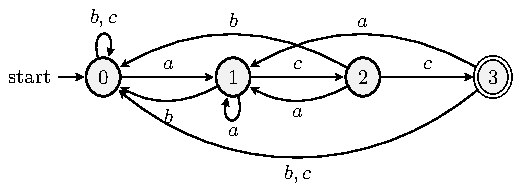
\includegraphics[width=0.35\textwidth]{./chapters/figures/forecasting/dfasr.pdf}
\label{fig:dfatcc}

\hfill

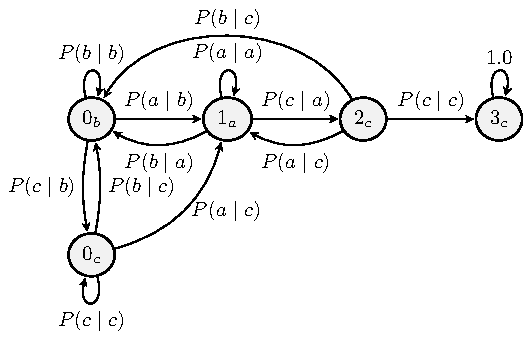
\includegraphics[width=0.35\textwidth]{./chapters/figures/forecasting/pmcr1.pdf}
\label{fig:mctcc1}

%\hfill
\caption{DFA and PMC for $\mathcal{P}=a ; c ; c$,  $\Sigma=\{a,b,c\}$, and order $m=1$  \cite{alevizos2017event}.}
\label{fig:dfa_mc_example}
\end{centering}
\end{figure}
%\end{comment}


\par After constructing a PMC, we can use it to calculate the so-called \textit{waiting-time} distributions.
Given a specific state of the PMC, a \textit{waiting-time} distribution gives us the probability of reaching a set of absorbing states in $n$ transition from now (absorbing states are states with self-loops and probability equal to $1.0$).
By mapping the final states of the initial DFA to absorbing states of the PMC
(see again Figure \ref{fig:dfa_mc_example}),
we can therefore calculate the probability of reaching a final state,
or, in other words, of detecting a full match of the original regular expression in $n$ events from now.

\par In order to estimate the final forecasts, another step is required,
since our aim is not to provide a single future point with the highest probability but an interval. 
Predictions are given in the form of intervals, like $I=(\mathit{start},\mathit{end})$. 
The meaning of such an interval is that the DFA is expected to reach a final state sometime in the future between $\mathit{start}$ and $\mathit{end}$ with probability at least some constant threshold $\theta_{fc}$ (provided by the user). 
These intervals are estimated by a single-pass algorithm that scans a waiting-time distribution and finds the smallest (in terms of length) interval that exceeds this threshold. 
An example is shown in Figure \ref{fig:wtdfas},
where the DFA in Figure \ref{fig:dfa1} is in state $1$,
the \textit{waiting-time} distributions for all of its non-final states are shown in Figure \ref{fig:wt1}
and the distribution, along with the prediction interval, for state $1$ are depicted in green.
\begin{figure}[!ht]
\begin{centering}

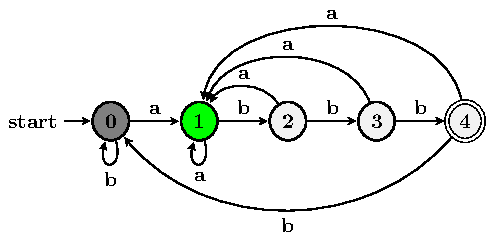
\includegraphics[width=0.19\textwidth]{./chapters/figures/forecasting/dfa1.pdf}
\label{fig:dfa1}


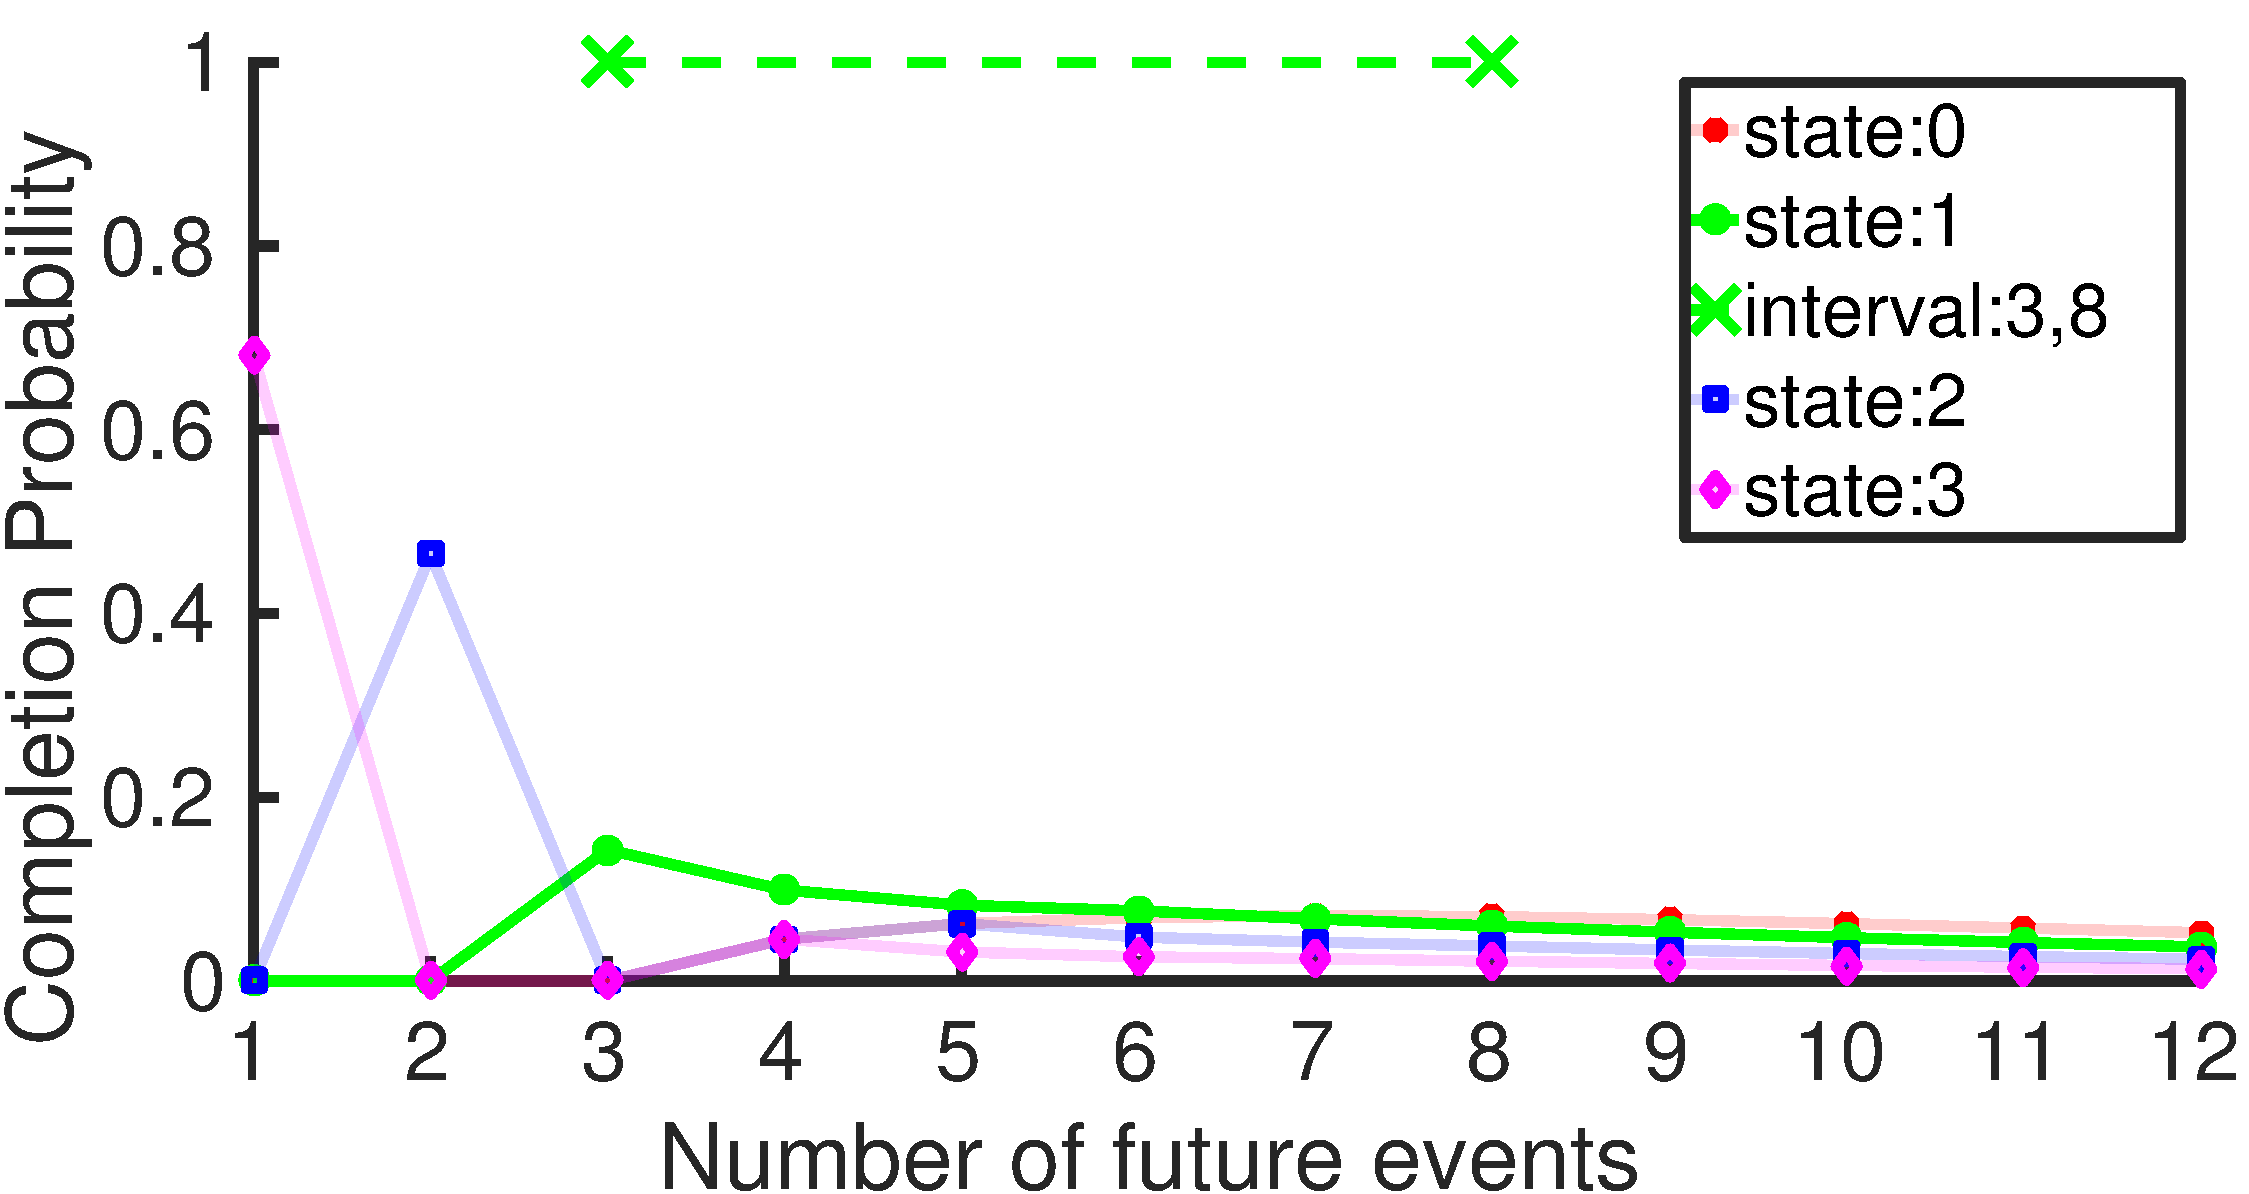
\includegraphics[width=0.28\textwidth]{./chapters/figures/forecasting/wt1.pdf}
\label{fig:wt1}

\caption{Example of how prediction intervals are produced. 
$\mathcal{P}=a ; b ; b ; b$, $\Sigma=\{a,b\}$, $m=1$, $\theta_{\mathit{fc}}=0.5$      \cite{alevizos2017event}.}
\label{fig:wtdfas}
\end{centering}
\end{figure}

\par The above described method assumes that we know the (possibly conditional) occurrence probabilities of the various event types appearing in a stream
(as would be the case with synthetically generated streams).
However, this is not always the case in real-world situations.
Therefore, it is crucial for a system implementing this method to have the capability to learn the values of the PMC's transition matrix.
One way to do this is to use some part of the stream to obtain the maximum-likelihood estimators for the transition probabilities as illustrated in Section ~\ref{sec:theoretical}. 

Executing this learning step on a single node might require a vast amount of time until we arrive at a sufficiently good model.
In this paper, we present a distributed method for learning the transition probability matrix.

\section{Pattern Prediction on multiple Streams}

\subsection{Problem Formulation}
Let $O = \{ o_1, ..., o_k\}$ be a set of \emph{$K$}  objects (i.e., moving objects) 
and $S = \{ s_1, ..., s_k\}$ a set of real-time streams of events,
where $s_i$ is generated by the object $o_i$.
Let $\mathcal{P}$ be a user-defined pattern which we want to apply to every stream $s_i$,
i.e., each object will have its own DFA.

\par The setting that is considered in this work is then described in the following:
we have \emph{$K$} input event streams $S$ and a system consisting of \emph{$K$} distributed predictor nodes $n_1,n_2...,n_k$, each of which consumes an input event stream $s_i\in S$. The goal is to provide timely predictions and be able to do this at large-scale.
Each node $n_i$ handles a single event stream $s_i$ associated with a moving object $o_i \in O$. In addition,  it  maintains a local prediction model $f_i$ for the user-defined pattern $\mathcal{P}$. The $f_i$ model provides the online prediction about the future full match of the pattern $\mathcal{P}$ in $s_i$  for each new arriving event tuple. 
\par In short, we have multiple running instances of an online prediction algorithm on distributed nodes for multiple input event streams. More specifically, the input to our system consists of massive streams of events  that describe trajectories of moving vessels in the context of maritime surveillance, where there is one predictor node for each vessel's event stream.
  
%
%The defined pattern $\mathcal{P}$ is monitored over each event stream $s_i$  by a  predictor nodes  $n_i$  that maintains a local prediction model $f_i$, where there is one node for each vessel's event stream.  The prediction model $f_i$ gives the ability to provide an online predictions about when the pattern will be completed in the form of an expected number of future events before a full match does occur.

\subsection{The Proposed Approach}
\label{sec:proposed_approach}
\par We designed and developed a scalable and distributed patterns prediction system over a massive input event streams of moving objects. As the base prediction model, we use the PMC forecasting method \cite{alevizos2017event}. Moreover,  we propose to enable the information exchange between the distributed predictors/learners of the input event streams, by adapting the distributed online prediction protocol of \cite{kamp2014communication} to synchronize the prediction models, i.e., the transitions probabilities matrix of the PMC predictors.

\par Algorithm~\ref{algonline:dol} presents the distributed online prediction protocol by dynamic model synchronization on both the predictor nodes and the coordinator. We refer to the PMC's transition matrix $\boldsymbol{\Pi}_i$ on predictor node $n_i$ by $f_i$. That is, when a predictor $n_i:\ i \in[k]$ observes an event $e_j$ it revises its internal model state (i.e., $f_i$) and provides a prediction report. Then it checks the local conditions  (batch size $b$ and local model divergence from a reference model $f_r$) to decide whether there is a need to synchronize its local model with the coordinator [or not].  $f_r$ is maintained in the predictor node as a copy of the last computed aggregated model $\hat{f}$ from the previous full synchronization step, which is shared between all local predictors/learners. By monitoring the local condition $\|f_i - f_r\|^2 > \Delta$ on all local predictors, we have a guarantee that if none of the local conditions is violated, the divergence (i.e., variance of local models $\delta(f)=\frac{1}{k} \sum_{j=1}^{k}\|f_i - \hat{f}\|^2$) does not exceed the threshold $\Delta$ \cite{kamp2014communication}. 

\par On the other hand, the coordinator receives the prediction models from the predictor nodes that requested for model synchronization (violation). Then it tries to keep incrementally querying other nodes for their local prediction models until reaching out all nodes, or the variance of the aggregated model $\hat{f}$ that is computed from the already received models less or equal than the divergence threshold  $\Delta$. Finally, the aggregated model $\hat{f}$ is sent back to the predictor nodes that sent their models after the violation or have been queried by the coordinator.

\begin{algorithm}[h]
	\caption{Communication-efficient Distributed Online Learning \cite{kamp2014communication}.} 
	\begin{algorithmic}[1] 
		\Statex \Indm  \textbf{Predictor} node $n_i$: at observing event $e_j$
		\Statex \Indp update the prediction model parameters $f_i$ and provide a prediction service \; 

		\Statex \If {$j\mod b = 0\ and\ \|f_i - f_r\|^2 > \Delta$}  
		\Statex send  $f_i$ to the Coordinator (violation) \;
		\Statex \Indm \textbf{Coordinator}:
		\Statex \Indp receive local models with violation 
		 $B=\{f_i\}_{i=1}^m$ \;
	
	
		\Statex \While{$|B| \neq k $ and $\frac{1}{|B|} \ \sum_{f_i\in  \Pi}\|f_i - \hat{f}\|^2 > \Delta$}{
			
			 \Statex  \hspace{\algorithmicindent} add other nodes have not reported violation for \Statex \hspace{\algorithmicindent} their models $ B \gets \{f_l : f_l \notin B\ and\ l \in [k]\}$    \;
			\Statex  \hspace{\algorithmicindent} receive models from nodes add to $B$\;
	}
        \Statex
		\Statex compute a new global model $\hat{f}$ \;
		\Statex send $\hat{f}$ to all the predictors in $B$ and set $f_{1}\dots f_{m}=\hat{f} $\; 
		\Statex \If {$|B| = k$}{
		\Statex  \hspace{\algorithmicindent} set a new reference model $f_r	\gets \hat{f}$ \; }
	
	\end{algorithmic}
	\label{algonline:dol}
\end{algorithm}


\par  We use this protocol for the pattern prediction model, which is internally based on the PMC \pmcmr. This allows the distributed \pmcmr\ predictors for multiple event streams to  synchronize their models (i.e., the transition probability matrix of each predictor) within the system in a communication-efficient manner. 



\par We propose a \textit{synchronization operation} for the parameters of the models ($f_i=\boldsymbol{\Pi}_i :i \in[k]$) of the $k$ distributed PMC predictors. The operation is based on distributing the maximum-likelihood estimation \cite{anderson1957statistical} for the transition probabilities of the underlying \pmcmr\ models described by: 
\begin{equation}
\label{eq:dis_pi_estim}
\hat{\pi}_{i,j}=\frac{\sum_{k \in K} n_{k,i,j}}{\sum_{k \in K} \sum_{l \in L} n_{k,i,l}}
\end{equation}

\par Moreover, we measure the divergence of local models from the reference model  $\|f_k - f_r\|^2$ by calculating the sum of square difference between the transition probabilities  $\boldsymbol{\Pi}_i$ and  $\boldsymbol{\Pi}_r$:
\begin{equation*}
\label{eq:dis_pi_varinace}
\|f_k - f_r\|^2=\sum_{i,j} (\hat{\pi}_k{i,j} -\hat{\pi}_r{i,j})^2
\end{equation*}
\par In general, our approach relies on enabling the collaborative learning between the prediction models of  the input event streams. By doing so, we assume that the underlying event streams belong to the same  distribution and share the same behavior (e.g., mobility patterns). We claim this assumption is reasonable in many application domains: for instance, in the context of maritime surveillance, vessels travel through standard routes, defined by the International Maritime Organization (IMO). Additionally, vessels have similar mobility patterns in specific areas such as moving with low speed and multiple turns near the ports \cite{pallotta2013vessel,liu2014knowledge}. That allows our system to construct a coherent global prediction model dynamically for all input event streams based on merging their local prediction models.

% may add it to conclusion 
%\par By enabling collaborative learning our approach is imposing an acceleration of learning of the underlying prediction models with less training data, in addition, it provides an improvement of the predictive performance compared to the no-distributed  version of event forecasting with Pattern Markov Chains system. 

\section{Analysis of the Proposed Approach}

\subsection{General  Overview}
\par Generally, our approach relies on enabling the collaborative learning among the distributed predictors. Each predictor node receives a stream of events related to a distinct moving object, and the central coordinator is responsible of synchronizing their prediction models using the \textit{synchronization operation}. Moreover, the predictors they only need to share the parameters of their models without aggregating all input event streams. 

\par In addition, our approach relies on enabling the collaborative learning between the prediction models of the input event streams. By doing so, we assume that the underlying event streams belong to the same  distribution and share the same behavior (e.g., mobility patterns). We claim this assumption is reasonable in many application domains: for example, in the context of maritime surveillance, vessels travel through standard routes, defined by the International Maritime Organization (IMO). Additionally, vessels have similar mobility patterns in specific areas such as moving with low speed and multiple turns near the ports \cite{pallotta2013vessel,liu2014knowledge}. That allows our system to construct a coherent global prediction model dynamically for all input event streams based on merging their local prediction models.

\par The underlaying learning process is based on estimating the transition probability matrix of the \pmcmr models, where the maximum-likelihood estimator  \cite{anderson1957statistical} is used to learn the transition probability matrix for each \pmcmr. In our approach, we propose a synchronization operation (Equation ~\ref{eq:dis_pi_estim}) to build a global estimation of the transition probability matrix among the \emph{$K$} predictors. In next, we present the maximum-likelihood estimator, and we  provide a theoretical analysis of the proposed operation, where we further present a probabilistic guarantee of the efficiency of our distributed learning estimation against the isolated estimations.   
% may add it to conclusion 
%\par By enabling collaborative learning our approach is imposing an acceleration of learning of the underlying prediction models with less training data, in addition, it provides an improvement of the predictive performance compared to the no-distributed  version of event forecasting with Pattern Markov Chains system. 


\subsection{Theoretical Analysis}
\label{sec:theoretical}

 In this section, we present preliminaries of the Markov chain models and the maximum-likelihood estimator of the transition probabilities, and we describe the theoretical properties of our proposed synchronization operator and its relation with the maximum-likelihood estimator. Also, we derive a probabilistic guarantee of our method estimations for the transition probabilities. 
 
 
 \subsubsection*{Preliminaries}
 We first give a brief introduction to the Markov chain theory, where the theoretical definitions and notations presented are based on the work described in \cite{bertsekas2002introduction,Billingsley1961,anderson1957statistical,howard2012dynamic}.

\begin{definition}
	Let $\{q_0, q_1, \ldots q_n\}$ be a sequence of random variables as \textbf{Markov chain}, where the variable $q_i$ belongs to a finite state space $\mathbf{S =\{1,\ldots m\}}$ and represents the observed state of the chain at time $i$. Let the transition probabilities of the Markov chain $p_{ij}(t+1)$ such that $i,j \in S$ and $t=0,\ldots, n$, where  $p_{ij}(t+1)$ is the probability of the state $j$ at time $t+1$, given  state $i$ at time $t$, then the sequence $\{q_0, q_1, \ldots q_n\}$ satisfies the \textbf{Markov property} 
	
	\begin{equation}
	\begin{aligned}
	P(q_{t+1}=j|q_{t}=i,q_{t-1}=i_{t-1},\ldots ,q_{0}=i_{0})=P(q_{t+1}=j|q_{t}=i)\\
	\forall i,j,i_{t-1},i_{0} \in S
	\end{aligned}
	\end{equation}

\end{definition}



\par That is, the probability of moving to a future state only depends on the current state (Markov chain of order $1$). While for higher order $m$ Markov chains the conditional probabilities are modeled to be dependent on the last $m$ states. 

\par When the conditional probabilities $P(q_{t+1}=j|q_{t}=i)$ are independent of the time $t$, the Markov chain is called \textbf{homogeneous} such that $p_{ij}:=P(q_{t+1}=j|q_{t}=i)$.

The transition probabilities of the Markov chain are represented by a $m \times m$ matrix that called \textbf{transition probability matrix} $\boldsymbol{\Pi}$ with $p_{ij}$ elements


\begin{equation}
\label{eq:matrix_example}
\boldsymbol{\Pi} = 
\begin{bmatrix} 
p_{1,1}	   &p_{1,2}  &. 		&. 		& . &  	p_{1,m} \\
p_{2,1}		   &.  & .		& .	    & .	& . \\
. 		   &.  & .		& .	    & .	& . \\
.		   &.  & .		& .		& .	& . \\
.		   &.  & .		& .		& .	& .\\
p_{m,1}	   & p_{m,1}	&.		& .	& .	&p_{m,m}
\end{bmatrix}
\end{equation}

where $0 \leq p_{i,j}\leq 1 $ and the rows sum up to one 
\begin{equation}
\sum_{j=1}^{m} p_{i,j}= 1\ \ \ \ \ \ \ \ \ i=1,2 \ldots m
\end{equation}

\subsection{Learning the Transition Probability Matrix for a Single Markov Chain}
 \
\par As mentioned in Section ~\ref{sec:pmc_prediction}, we rely on the transition probability matrix of \pmcmr to build the prediction intervals. Given that the sequence of the states $\{q_0, q_1, \ldots q_n\}$ that DFA visits after consuming the input event stream is a 1-order Markov chain.


\par However, in practice the underlying transition probability matrix is unknown, and desirable to estimate or learn it form the observed sequence $\{q_0, q_1, \ldots q_n\}$. The maximum-likelihood estimator is a common method to estimate the transition probability matrix \cite{anderson1957statistical}.


\begin{definition}
	Let $\boldsymbol{\Pi}$ is the transition probability matrix of a single Markov chain with a set of states $S$, 
	$\pi_{i,j}$ the transition probability from state $i$ to state $j$,
	$n_{i,j}$ the number of observed transitions from state $i$ to state $j$,
	then the maximum-likelihood finds $\boldsymbol{\hat{\Pi}}$ as an estimate for $\boldsymbol{\Pi}$, where its elements $\hat{p}_{i,j}$ are
	\begin{equation}
	\label{eq:pi_estim}
	\hat{p}_{i,j}=\frac{n_{i,j}}{\sum_{l \in S} n_{i,l}}=\frac{n_{i,j}}{n_{i}}
	\end{equation}
	
\end{definition} 

Where this estimator is used separately to learn each transition probability matrix of all \pmcmr models.   


\textbf{Proprieties of the maximum-likelihood estimates}. 
	The maximum likelihood estimates of transition probabilities of a single sequence $\{q_0, q_1, \ldots q_n\}$  are obtained based on the observed transitions between the states of the chain. That is, the maximum likelihood estimates are basically the count of transitions from $i$ to $j$ divided by the total count of the chain being in state $i$.  
	
	\par ~\citet{anderson1957statistical} have shown that 
	
	
%	\begin{equation}
%	\label{eq:lim_dist}
%	\lim_{n\to\infty} \sqrt{n}\ (\hat{p}_{i,j} - {p}_{i,j}) \sim \mathcal{N}(\mu,\,\sigma^{2}_{mle})\,.
%	\end{equation}

	\begin{equation}
	\begin{aligned}
	\label{eq:lim_dist}
	 \sqrt{n}\ (\hat{p}_{i,j} - {p}_{i,j}) \xrightarrow{d} \mathcal{N}(\mu,\,\sigma^{2})\\
	 as\ n \xrightarrow{} \infty
	 \end{aligned}
	\end{equation}
Thus, the random variable $\sqrt{n}\ (\hat{p}_{i,j} - {p}_{i,j})$ has asymptotically normal distribution with mean $\mu=0$, and  variance  $\sigma^{2}$ is given by   

\begin{equation}
\begin{aligned}
\sigma^{2}=\mathrm{Var}(\sqrt{n}\ (\hat{p}_{i,j} - {p}_{i,j})) = \frac {{p}_{i,j}\ (1- {p}_{i,j})} {\phi_{i}} \\
\text{s.t.}\ \phi_{i} = \sum_{l=1}^{m} \sum_{t=1}^{n} \eta_{l} \ p_{l,j}^{t-1}
\end{aligned}
\end{equation}

Where $p_{l,j}^{t-1}$ is the probability of state $j$ at time $t-1$ given that the state $l$ at time $0$ ~\cite{anderson1957statistical}. We are interested in the variances of $(\hat{p}_{i,j} - {p}_{i,j})$ that represents the error in the estimation of ${p}_{i,j}$ by the maximum-likelihood estimator, which is given by:

	\begin{equation}
\begin{aligned}
\label{eq:var_isol}
	\mathrm{Var} (\hat{p}_{i,j} - {p}_{i,j}) =  \frac {\mathrm{Var}(\sqrt{n}\ (\hat{p}_{i,j} - {p}_{i,j}))}{n} = \frac {\sigma^{2}}{n} 
\end{aligned}
\end{equation}

It is clearly seen that variances are dropping as the sample size $n$ grows large.  In next, we will show that our proposed approach of synchronizing the maximum likelihood estimators over $k$ chains is preserving  a similar asymptotic behavior and gives efficient estimates of the transition probabilities.


\subsubsection{Probabilistic Learning Guarantee}
 %in Equation ~\ref{eq:dis_pi_estim}% 
\par The proposed synchronization operator is aggregating the maximum-likelihood estimates over $k$ observed sequences (i.e., sequences of the DFA states based on the consumed event streams), the operator estimates a global transition probabilities matrix for a set of $k$ sequences, which are arranged in serial order as one large chain with length $N=k*n$, where we assume that all $k$ sequences have $n$ observations. For the sake of simplicity, we assume that the synchronization phase happens on batch size equals $n$ (i.e., $b=n$) given that the $\Delta$ is zero, then the global transition probabilities $\hat{\pi}_{i,j}$ are given 
\begin{equation}
\label{eq:dis_pi_estim2}
	\begin{aligned}
\hat{\pi}_{i,j}=\frac{\sum_{k \in K} n_{k,i,j}}{\sum_{k \in K} \sum_{l \in L} n_{k,i,l}} = \hat{p}_{i,j}(N)\\\\
 where\ N = k*n.
 \end{aligned}
\end{equation}
%This is equivalent to

\par Thus, this operation it allows to observe more samples, which is naturally producing a better estimates of the transition probabilities. In addition, our proposed synchronization operation of the $k$ transition matrices has the same proprieties as the maximum likelihood estimator over a serial sequence of all $k$ sequences, but with skipping $k-1$ transitions between each two consecutive sequences, which is in practice a small number that can be neglected comparing to the total transitions count $k*n$. As result, the global transition probabilities of our approach  have the same properties as maximum likelihood estimates, in particular, the the random variable $\sqrt{N}\ (\hat{\pi}_{i,j} - {p}_{i,j})$ has asymptotically normal distribution with mean $\mu=0$, and  following Equation ~\ref{eq:lim_dist} we have variance 

\begin{equation}
\begin{aligned}
\label{eq:lim_dist2}
\sqrt{N}\ (\hat{\pi}_{i,j} - {p}_{i,j}) \xrightarrow{d} \mathcal{N}(0,\,\sigma^{2})\\
as\ N \xrightarrow{} \infty\\
where\ N = n*k .\\
\end{aligned}
\end{equation}

So, 
\begin{equation}
\begin{aligned}
\label{eq:var_sync}
 \mathrm{Var} (\hat{\pi}_{i,j} - {p}_{i,j}) = \frac {\sigma^{2}}{N} =  \frac {\sigma^{2}}{k*n}
\end{aligned}
\end{equation}


That is, since $N > n$ combining $k$ sequences, the variances of estimations of our method  $\mathrm{Var} (\hat{\pi}_{i,j} - {p}_{i,j})$ are smaller than the estimates of maximum-likelihood over a single sequence $\mathrm{Var} (\hat{p}_{i,j} - {p}_{i,j})$. 
\par Thus, it follows from the  Chebyshev's inequality \cite{feller1968introduction} that we have for the random variable $\hat{p}_{i,j} - {p}_{i,j}$, for any constant $c > 0$  

\[ \Pr\left( |(\hat{p}_{i,j} - {p}_{i,j}) - \mu| \geq c \right) \leq
\frac{\mathrm{Var} (\hat{p}_{i,j} - {p}_{i,j})}{c^2} \]


 The mean $\mu=0$ is zero and the $\mathrm{Var} (\hat{p}_{i,j} - {p}_{i,j})$ equals  $\frac {\sigma^{2}}{n}$, and therefore 
 
 \[ \Pr\left( |\hat{p}_{i,j} - {p}_{i,j}| \geq c \right) \leq
 \frac{\sigma^{2}}{c^2 * n} \]
 
 
$\hat{p}_{i,j} - {p}_{i,j}$  represents the deviation/error between the estimates of maximum-likelihood over a single (i.e., isolated) sequence and the true probabilities. On the other hand, we can obtain, in the same way, the probability bound of deviations for our synchronization operator estimates as follows:

\[ \Pr\left( |\hat{\pi}_{i,j} - {p}_{i,j}| \geq c \right) \leq
\frac{\sigma^{2}}{c^2* n*k} \]


\par Using Equation~\ref{eq:var_sync} we obtain the value $\mathrm{Var} (\hat{\pi}_{i,j} - {p}_{i,j})$, and Equation~\ref{eq:var_sync} for $\mathrm{Var} (\hat{p}_{i,j} - {p}_{i,j})$. Given that $k \ge 1$, then  the variance of $\hat{\pi}_{i,j} - {p}_{i,j}$  is less than or equal to the variance of $\hat{p}_{i,j} - {p}_{i,j}$

\[ 
\frac{\sigma^{2}}{c^2 *n*k} \leq
\frac{\sigma^{2}}{c^2 * n}
 \]

So, we have for any constant $c > 0$ and $k \ge 1$, a probabilistic learning guarantee of the transition probabilities: 

\[ \Pr\left( |\hat{\pi}_{i,j} - {p}_{i,j}| \geq c \right) \leq
 \Pr\left( |\hat{p}_{i,j} - {p}_{i,j}| \geq c \right)
 \]
 where $\hat{p}_{i,j}$ a transition probability, which is learned on a single \pmcmr predictor, and the $\hat{\pi}_{i,j}$ is the global transition probability that computed by the synchronization operation (Equation ~\ref{eq:dis_pi_estim}). To summarize, our approach is based aggregating the maximum-likelihood estimates over $k$ sequences, which speeds up the convergence to reach the true transition probabilities as result of the smaller variances of the estimates.

%The weak law of large
%numbers states that, if $X_1, X_2, X_3, \ldots$ are independent and identically
%distributed random variables with mean $\mu$ and standard deviation $\sigma$,
%then for any constant $\epsilon > 0$ we have 
%%
%\[ \lim_{n \rightarrow \infty} \Pr \left( \left| \frac{X_1 + X_2 + \cdots +
%	X_n}{n} - \mu \right| > \epsilon \right) = 0. \]
%Use Chebychev's inequality to prove the weak law of large numbers.

 
\subsection{Transition Matrix of the Underlaying Markov Chain}
\label{sec:underlaying_mc}
\par In order to empirically study the learning efficiency of our distributed learning based proposed approach against the isolated approach, we need to map the transition probabilities of the underlying Markov chain with the transition probability matrix ($\hat{\Pi}$) of the \pmcmr model. ~\citet{nuel_pattern_2008} showed in \textbf{Theorem 3} the relation between the elements  of 
$\Pi$ and the conditional probabilities of the $m-$order Markov chain $X=\{X_1, X_2, \ldots X_n\}$ described by 

\[ \Pi(p, q) =
\begin{cases}
P(X_{m+1}=b|X_1\ldots X_m=\delta^{-m}(p))     & \quad \text{if } \delta(p,q)=b \\
0  & \quad \text{if } p \notin  \delta(p,X)
\end{cases}
\]
Using this theorem, in the case of the underlaying transition probability matrix is known (e.g., synthetic event streams),  we then can compare the estimation efficiency of the different approaches for the transition probabilities of the underlaying Markov chain $X$.  For example, the transition probability matrix of the \pmcmr model for the pattern $\mathcal{P}=a ; d ; c$ over  $\Sigma=\{a,b,c,d\}$ is represented by: 

\begin{equation}
\label{eq:matrix}
\boldsymbol{\Pi} = 
\begin{Bmatrix} 
 1          \\ 2        \\3             \\4         \\5         \\ 6 
\end{Bmatrix}
\begin{bmatrix} 
P(a|a) 	& P(b|a) 		& P(c|a) 		& 0			  & p(d|a) 	& 0  \\
P(a|b) 	& P(b|b) 		& P(c|b) 		& P(d|b)	  & 0 	    & 0  \\
P(a|c) 	& P(b|c) 		& P(c|c) 		& P(d|c) 	  & 0 	    & 0  \\
P(a|d) 	& P(b|d) 		& P(c|d) 		& P(d|d)	  & 0 	    & 0  \\
P(a|d) 	& P(b|d) 		&  0	 	    & P(d|d)	  & 0 	    & P(c|d)  \\
0			& 0			& 0		        & 0    		  & 0		& 1.0
\end{bmatrix}
\end{equation} 

%ADD figure example for the figure in the PMC section%